\section*{Experimental Design}
The task that trial subjects were faced with was designed to facilitate
comparison between the subjects' decisions those that would be made by a
Bayesian algorithm. Modeling a sequential online categorization was useful both
because that was the type of categorization algorithm developed in previous
work, and because it had a straightforward manifestation in a constrained human
task. Trial subjects were presented with stimuli images, sequentially, and asked
to sort each image as it appeared into a group. Once the image was placed in a
group, the subject was not allowed to switch the image to another group.  The
instructions given to each subject can be viewed in the Appendix, Figure
\ref{fig:instructions}. 

The stimuli used were 10-by-10 pixelated images. Each pixel-block in the image
was a colored between white and black, with 256 possible grayscale values. These
type of images were chosen to both make the task difficult for the human subject and
to make the input data directly interpretable for the inference algorithm.
Figure \ref{fig:clusterer} shows a mostly completed trial.

Workers on Mechanical Turk were hired to be trial subjects. They were presented
with a website to conduct the trial on: each worker was first shown the
instruction page in Figure \ref{fig:instructions}, and then were brought to the
page on which the trial was conducted, show in Figure \ref{fig:clusterer}  All
the actions performed by the subject were collected in a database to be used for
later analysis.

\begin{figure}
\centering
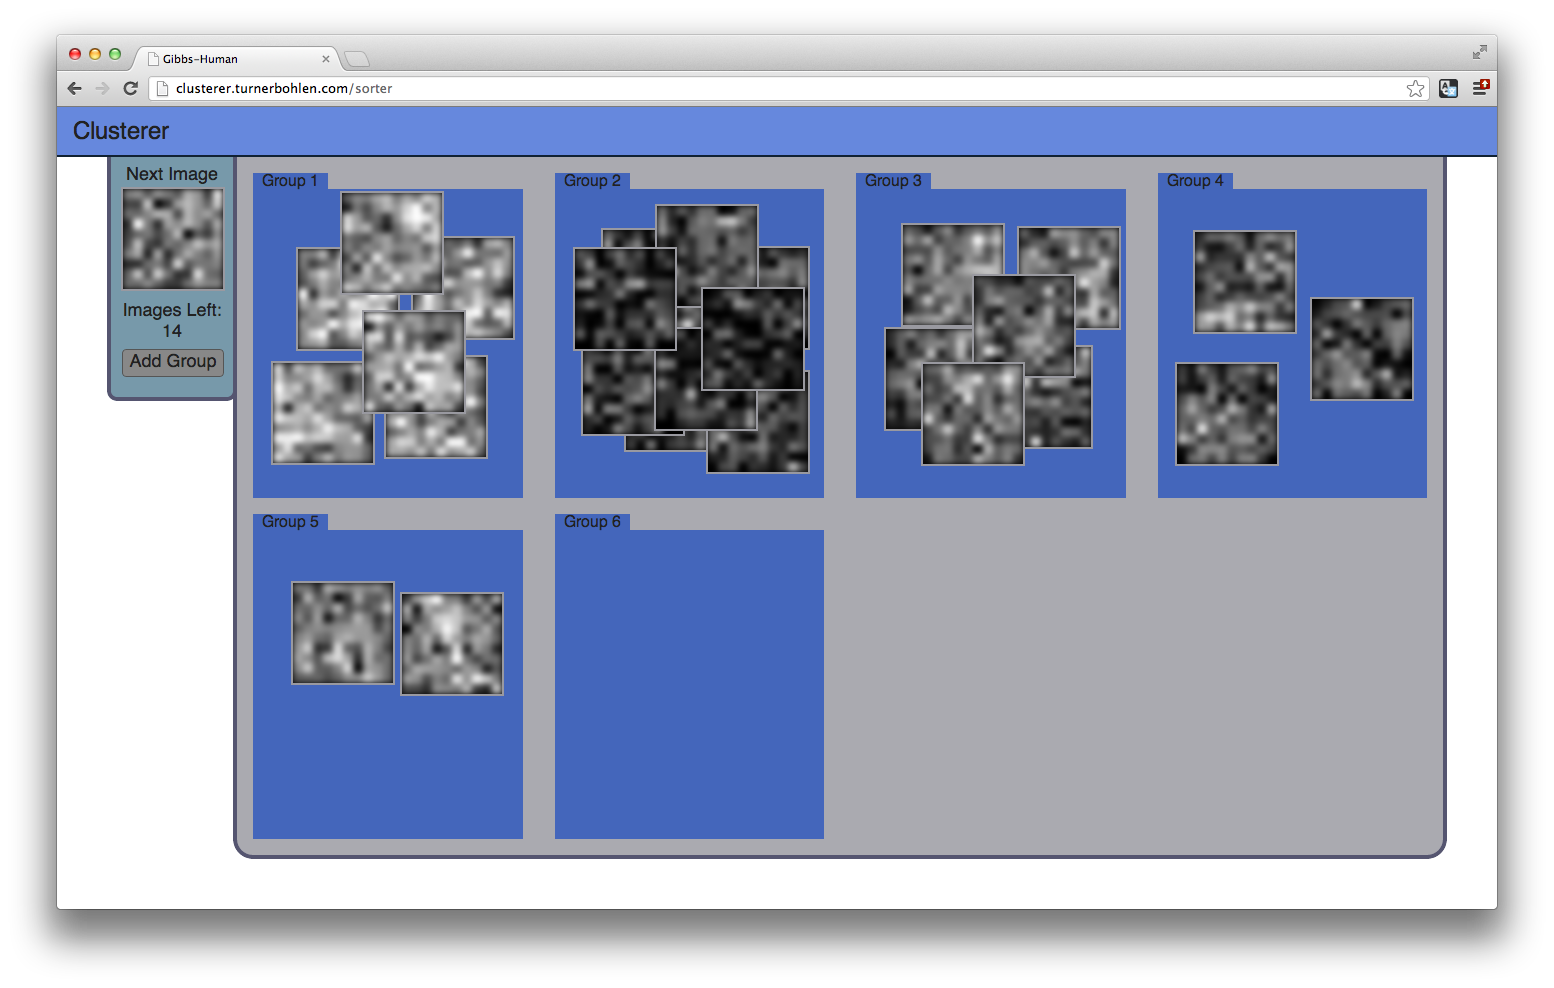
\includegraphics[width=5.6in]{img/clusterer.png}
\label{fig:clusterer}
\caption{Interface through which a trial was completed. Images are dragged from
  the 'Next Image' box into one of the groups. Once an image was placed in a
  group, it could not be switched into another group.  The subject was limited
  to creating 8 groups.}
\end{figure}